\documentclass[]{exam}
\usepackage{epic,array,ecltree,url,calrsfs}
\usepackage[nointegrals]{wasysym}
\usepackage{mlextra}

%These tell TeX which packages to use.
\usepackage{array,epsfig}
\usepackage{amsmath}
\usepackage{amsfonts}
\usepackage{amssymb}
\usepackage{amsxtra}
\usepackage{amsthm}
\usepackage{mathrsfs}
\usepackage[dvipsnames]{xcolor}
\usepackage{array}
\usepackage{graphicx}
\graphicspath{ {../art/} }
\usepackage{bm}
\usepackage{tikz}
\usepackage{multicol}
\usepackage{enumitem}

\renewcommand\qedsymbol{$\blacksquare$}

%Here I define some theorem styles and shortcut commands for symbols I use often
%\theoremstyle{definition}
%\newtheorem{defn}{Definition}
%\newtheorem{thm}{Theorem}
%\newtheorem{cor}{Corollary}
%\newtheorem*{rmk}{Remark}
%\newtheorem{lem}{Lemma}
%\newtheorem*{joke}{Joke}
%\newtheorem{ex}{Example}
%\newtheorem*{soln}{Solution}
%\newtheorem{prop}{Proposition}

\newcommand{\lra}{\longrightarrow}
\newcommand{\ra}{\rightarrow}
\newcommand{\surj}{\twoheadrightarrow}
\newcommand{\graph}{\mathrm{graph}}
\newcommand{\bb}[1]{\mathbb{#1}}
\newcommand{\Ell}{\mathscr{L}}
\newcommand{\Z}{\bb{Z}}
\newcommand{\Q}{\bb{Q}}
\newcommand{\R}{\bb{R}}
\newcommand{\C}{\bb{C}}
\newcommand{\N}{\bb{N}}
\newcommand{\M}{\mathbf{M}}
\newcommand{\m}{\mathbf{m}}
\newcommand{\MM}{\mathscr{M}}
\newcommand{\HH}{\mathscr{H}}
\newcommand{\Om}{\Omega}
\newcommand{\Ho}{\in\HH(\Om)}
\newcommand{\bd}{\partial}
\newcommand{\del}{\partial}
\newcommand{\bardel}{\overline\partial}
\newcommand{\textdf}[1]{\textbf{\textsf{#1}}\index{#1}}
\newcommand{\img}{\mathrm{img}}
\newcommand{\ip}[2]{\left\langle{#1},{#2}\right\rangle}
\newcommand{\inter}[1]{\mathrm{int}{#1}}
\newcommand{\exter}[1]{\mathrm{ext}{#1}}
\newcommand{\cl}[1]{\mathrm{cl}{#1}}
\newcommand{\ds}{\displaystyle}
\newcommand{\vol}{\mathrm{vol}}
\newcommand{\cnt}{\mathrm{ct}}
\newcommand{\osc}{\mathrm{osc}}
\newcommand{\LL}{\mathbf{L}}
\newcommand{\UU}{\mathbf{U}}
\newcommand{\support}{\mathrm{support}}
\newcommand{\AND}{\;\wedge\;}
\newcommand{\OR}{\;\vee\;}
\newcommand{\Oset}{\varnothing}
\newcommand{\st}{\ni}
\newcommand{\wh}{\widehat}

%Pagination stuff.
\setlength{\topmargin}{-.3 in}
\setlength{\oddsidemargin}{0in}
\setlength{\evensidemargin}{0in}
\setlength{\textheight}{9.in}
\setlength{\textwidth}{6.5in}

\newcommand{\id}[1]{\mbox{\it #1\/}}
\newcommand{\rid}[1]{\mbox{\rm #1}}
\newcommand{\sid}[1]{\mbox{\sf #1}}
\newcommand{\bid}[1]{\mbox{\bf #1}}
\newcommand{\tinysz}[1]{\mbox{\tiny $#1$}}

\newtheorem{innerdefn}{Definition}
\newenvironment{defn}[1]
  {\renewcommand\theinnerdefn{#1}\innerdefn}
  {\endinnerdefn}

\newtheorem{innerexample}{Example}
\newenvironment{ex}[1]
  {\renewcommand\theinnerexample{#1}\innerexample}
  {\endinnerexample}

\newtheorem{innerthm}{Theorem}
\newenvironment{thm}[1]
  {\renewcommand\theinnerthm{#1}\innerthm}
  {\endinnerthm}



\newcommand{\twonode}{%
  \begingroup\normalfont
  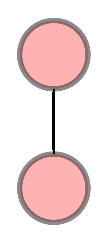
\includegraphics[height=\fontcharht\font`\b]{2nodetree.eps}%
  \endgroup
}


\title{Lab 5: Validity, Satisfiability, Normal Forms}
\author{Foundations of Computer Science}
\date{\today}
%\pagestyle{empty} 
%\footer{}{\thepage}{}
\printanswers
\unframedsolutions
\SolutionEmphasis{\itshape\small}
\SolutionEmphasis{\color{NavyBlue}}


\begin{document}

\maketitle

\setlength{\columnseprule}{1pt}
\begin{questions}

\question Answer the questions below for the formula $A$, where $A \equiv (p \implies q)
  \eqv (\ngg p \implies \ngg q)$.
\begin{parts}
\part What is $\mathcal{P}_A$? 
\begin{solution}
$\{p,q \}$
\end{solution}

\part Define $\mathcal{I}_A: \mathcal{P}_A \to \{T,F\}$ as $\mathcal{I}_A(p) =
T$, $\mathcal{I}_A(q) = F$.  Is $\mathcal{I}_A$ a model for $A$?
\begin{solution}
No.
\end{solution}

\part Given an interpretation that satisfies $A$ or prove $A$ is not
satisfiable.
\begin{solution}
$\mathcal{I}_A(p) = T$, $\mathcal{I}_A(q) = T$ or $\mathcal{I}_A(p) = F$, $\mathcal{I}_A(q) = F$ \\
\end{solution}
\end{parts}


\question Answer the questions below for the formula $A$, where $A \equiv (p \implies q) \implies q) \implies q$.
\begin{parts}
\part What is $\mathcal{P}_A$? 
\begin{solution}
$\{p,q \}$
\end{solution}

\part Define $\mathcal{I}_A: \mathcal{P}_A \to \{T,F\}$ as $\mathcal{I}_A(p) =
T$, $\mathcal{I}_A(q) = T$.  Is $\mathcal{I}_A$ a model for $A$?
\begin{solution}
Yes.
\end{solution}

\part Is $A$ satisfiable?
\begin{solution}
Yes.
\end{solution}

\part Prove $\models A$ or give an interpretation that falsifies $A$.
\begin{solution}
$\mathcal{I}_A(p) = T$, $\mathcal{I}_A(q) = F$ or $\mathcal{I}_A(p) = F$, $\mathcal{I}_A(q) = T$
\end{solution}
 
\end{parts}

\question Answer the questions below for the formula $A$, where $A \equiv (p \eqv q) \eqv (q \eqv (q \eqv p))$.
\begin{parts}
\part Give an interpretation that satisfies $A$.
\begin{solution}
$\mathcal{I}_A(p) = T$, $\mathcal{I}_A(q) = T$ or $\mathcal{I}_A(p) = T$, $\mathcal{I}_A(q) = F$
\end{solution}
\part Prove $A$ is valid or give an interpretation that falsifies $A$.
\begin{solution}
$\mathcal{I}_A(p) = F$, $\mathcal{I}_A(q) = F$ or $\mathcal{I}_A(p) = F$, $\mathcal{I}_A(q) = T$
\end{solution}
\end{parts}

\question Answer the questions below for the formula $A$, where $A \equiv ((p \land q) \implies
    r) \implies ((p \implies r) \lor (q \implies r))$ 
\begin{parts}
\part Change $A$ to Negative Normal Form. 
\begin{solution}
~\\
%$((p \land q) \implies r) \implies ((p \implies r) \lor (q \implies r))$\\
%$(\ngg (p \land q) \lor r) \implies ((\ngg p \lor r) \lor (\ngg q \lor r))$\\
%$\ngg (\ngg (p \land q) \lor r) \lor ((\ngg p \lor r) \lor (\ngg q \lor r))$\\
%$ ( (p \land q) \land \ngg r) \lor ((\ngg p \lor r) \lor (\ngg q \lor r))$\\
$ ((p \land q) \land \ngg r) \lor (\ngg p \lor r \lor \ngg q)$\\

\end{solution}
\part Change $A$ to Conjunctive Normal Form.
\begin{solution}
%$ ( (p \land q) \land \ngg r) \lor ((\ngg p \lor r) \lor (\ngg q \lor r))$\\
%$ ( (p \land q)\lor (\ngg p \lor r \lor \ngg q )) \land (\ngg r \lor (\ngg p \lor r \lor \ngg q )) $\\
$ (p \lor \ngg p \lor r \lor \ngg q ) \land (q \lor \ngg p \lor r \lor \ngg q  ) \land (\ngg r \lor \ngg p \lor r \lor \ngg q ) $\\
\end{solution}
\part Prove $\models A$.
\begin{solution}
$A \equiv (p \lor \ngg p \lor r \lor \ngg q ) \land (q \lor \ngg p \lor r \lor \ngg q  ) \land (\ngg r \lor \ngg p \lor r \lor \ngg q ) $\\
$((p \lor \ngg p) \lor r \lor \ngg q) \equiv 
           (\top \lor r \lor \ngg q ) \equiv \top$ \\
$(q \lor \ngg p \lor r \lor \ngg q )  \equiv 
 ((q \lor \ngg q) \lor \ngg p \lor r) \equiv 
           (\top \lor \ngg p \lor r ) \equiv \top$ \\
  $(\ngg r \lor \ngg p \lor r \lor \ngg q ) \equiv 
 ((\ngg r \lor r) \lor \ngg p \lor \ngg q ) \equiv 
            (\top \lor \ngg p \lor \ngg q ) \equiv \top$\\
Therefore, $A \equiv \top \land \top \land \top \equiv \top$ 
\end{solution}
\part Show that $\ngg A$ is unsatisfiable.
\begin{solution}
By theorem (2.39) in Ben Ari, $\ngg A$ is unsatisfiable if and only if $A$ is
valid. We have proved that $A$ is valid in the previous problem, so $\ngg A$ is unsatisfiable.

\end{solution}
\end{parts}

\question Answer the questions below for the formula $A$, where $A \equiv (p \implies q) \lor (q \implies r)$ 
\begin{parts}
\part Change $A$ to Negative Normal Form. 
\begin{solution}
~\\
$A \equiv (p \implies q) \lor (q \implies r)$\\
$ \equiv (\ngg p \lor q) \lor (\ngg q \lor r)$
\end{solution}
\part Change $A$ to Conjunctive Normal Form.
\begin{solution}
$A \equiv (\ngg p \lor q) \lor (\ngg q \lor r)$ 
$\equiv (\ngg p \lor q \lor \ngg q \lor r) $
\end{solution}
\part Prove $\models A$.
\begin{solution}
$A \equiv (\ngg p \lor q \lor \ngg q \lor r) 
  \equiv (\ngg p \lor (q \lor \ngg q) \lor r)
  \equiv (\ngg p \lor \top \lor r)
  \equiv \top$
\end{solution}
\part Show that $\ngg A$ is unsatisfiable.
\begin{solution}
Again, by theorem (2.39) in Ben Ari, $\ngg A$ is unsatisfiable if and only if $A$ is
valid. 
\end{solution}
\end{parts}

\question Change $A$ to Conjunctive Normal Form. 
\begin{parts}
\part\label{q:4lit} $A \equiv (p_1 \land q_1) \lor (p_2 \land q_2)$.
\begin{solution}
~\\
$A \equiv (p_1 \land q_1) \lor (p_2 \land q_2)$.\\
$\equiv ((p_1 \lor (p_2 \land q_2)) \land (q_1 \lor (p_2 \land q_2)$.\\
$\equiv (p_1 \lor p_2) \land (p_1 \lor q_2) \land (q_1 \lor p_2) \land (q_1 \lor q_2)$.\\
\end{solution}
\part\label{q:6lit} $A \equiv (p_1 \land q_1) \lor (p_2 \land q_2) \lor (p_3 \land q_3)$.
\begin{solution}
~\\
$A \equiv (p_1 \land q_1) \lor (p_2 \land q_2) \lor (p_3 \land q_3)$.\\
$\equiv ((p_1 \lor p_2) \land (p_1 \lor q_2) \land (q_1 \lor p_2) \land (q_1 \lor q_2)) \lor (p_3 \land q_3)$. (by part (a) above)\\
$\equiv ((p_1 \lor p_2) \land (p_1 \lor q_2) \land (q_1 \lor p_2)) \land (q_1 \lor q_2) \lor (p_3 \land q_3)$.

$\equiv (((p_1 \lor p_2) \land (p_1 \lor q_2) \land (q_1 \lor p_2)) \lor (p_3 \land q_3)) 
  \land ((q_1 \lor q_2) \lor (p_3 \land q_3))$.
  
$\equiv (((p_1 \lor p_2) \land (p_1 \lor q_2) \land (q_1 \lor p_2)) \lor (p_3 \land q_3)) 
  \land (((q_1 \lor q_2) \lor p_3) \land ((q_1 \lor q_2) \lor q_3))$.

$\equiv (((p_1 \lor p_2) \land (p_1 \lor q_2)) \land (q_1 \lor p_2) \lor (p_3 \land q_3)) 
  \land (q_1 \lor q_2 \lor p_3) \land (q_1 \lor q_2 \lor q_3)$.

$\equiv (((p_1 \lor p_2) \land (p_1 \lor q_2)) \lor (p_3 \land q_3))
  \land ((q_1 \lor p_2) \lor (p_3 \land q_3)) 
  \land ((q_1 \lor q_2 \lor p_3) \land (q_1 \lor q_2 \lor q_3)$.

$\equiv (((p_1 \lor p_2) \land (p_1 \lor q_2)) \lor (p_3 \land q_3)) 
  \land (((q_1 \lor p_2) \lor p_3 \land (q_1 \lor p_2) \lor q_3)) 
  \land ((q_1 \lor q_2 \lor p_3) \land (q_1 \lor q_2 \lor q_3)$.

$\equiv ((p_1 \lor p_2) \land (p_1 \lor q_2) \lor (p_3 \land q_3)) 
  \land ((q_1 \lor p_2 \lor p_3) \land (q_1 \lor p_2 \lor q_3)) 
  \land ((q_1 \lor q_2 \lor p_3) \land (q_1 \lor q_2 \lor q_3)$.

$\equiv ((p_1 \lor p_2) \lor (p_3 \land q_3)) 
  \land ((p_1 \lor q_2) \lor (p_3 \land q_3)) 
  \land ((q_1 \lor p_2 \lor p_3) \land (q_1 \lor p_2 \lor q_3)) 
  \land ((q_1 \lor q_2 \lor p_3) \land (q_1 \lor q_2 \lor q_3)$.

$\equiv ((p_1 \lor p_2) \lor p_3 \land q_3) 
  \land ((p_1 \lor q_2) \lor p_3 \land q_3) 
  \land ((q_1 \lor p_2 \lor p_3) \land (q_1 \lor p_2 \lor q_3)) 
  \land ((q_1 \lor q_2 \lor p_3) \land (q_1 \lor q_2 \lor q_3)$.

$\equiv ((p_1 \lor p_2) \lor p_3 \land (p_1 \lor p_2) \lor q_3) 
  \land ((p_1 \lor q_2) \lor p_3 \land (p_1 \lor q_2) \lor q_3) 
  \land ((q_1 \lor p_2 \lor p_3) \land (q_1 \lor p_2 \lor q_3)) 
  \land ((q_1 \lor q_2 \lor p_3) \land (q_1 \lor q_2 \lor q_3)$.

$\equiv (p_1 \lor p_2 \lor p_3) \land (p_1 \lor p_2 \lor q_3) 
  \land (p_1 \lor q_2 \lor p_3) \land (p_1 \lor q_2 \lor q_3) 
  \land (q_1 \lor p_2 \lor p_3) \land (q_1 \lor p_2 \lor q_3) 
  \land (q_1 \lor q_2 \lor p_3) \land (q_1 \lor q_2 \lor q_3)$.


\end{solution}
\end{parts}

\question Let $A$ be a formula of the form $(p_1 \land q_1) \lor (p_2 \land
    q_2)\lor ...\lor (p_n \land q_n)$
\begin{parts}
\part In terms of $n$, how many literals are in $A$?
\begin{solution}
$2n$
\end{solution}
\part Based on the pattern observed in the previous question, how many literals
will be in the CNF of $A$ (in terms of $n$)?
\begin{solution}
$n(2^n)$
\end{solution}
\end{parts}
\question  Using the modified version of the \texttt{Inorder} Function and
the formula \texttt{F1} given below, write the output of \texttt{Inorder(F1,0)}.
List all the calls to \texttt{Inorder} in the order they are made, with the
arguments passed in for each call. (You may want to label subformulas of
\texttt{F1}.)
\begin{verbatim}
Inorder(F,n)
  if F is a leaf
    write its label
    write `['
    write the value of n
    write `]'
    return
  let F1 and F2 be the left and right subtrees of F
  write a left parenthesis `('
  Inorder(F1, n+1)
  write the label of the root of F
  write `['
  write the value of n
  write `]'
  Inorder(F2, n+1)
  write a right parenthesis `)'
\end{verbatim}

\texttt{F1}  \\
\setlength{\GapWidth}{8mm}
\setlength{\GapDepth}{8mm}
\begin{bundle}{$\eqv$}
\chunk{
  \begin{bundle}{$\imp$}
  \chunk{$p$}
  \chunk{$q$}
  \end{bundle}
}
\chunk{
  \begin{bundle}{$\imp$}
  \chunk{
    \begin{bundle}{$\ngg$}
    \chunk{$p$}
    \end{bundle}
  }
  \chunk{
    \begin{bundle}{$\ngg$}
    \chunk{$q$}
    \end{bundle}
  }
  \end{bundle}
}
\end{bundle}\\
\begin{solution}
Let $FL_{\imp}$ and $FR_{\imp}$ refer to the left and right subtrees with $\imp$ as their
primary operator, and $FL_{\ngg}$ and $FR_{\ngg}$ refer to the left and right
subtrees with $\ngg$ as their primary operator. The following table enumerates
the function calls and their arguments on the left. The list on the right shows
the output printed after the function call with the same number on the left, but
before the next function call.
\begin{multicols}{2}
{ \bf Function Calls:}

\begin{enumerate}
\item \texttt{Inorder(F1,0)}
\item \texttt{Inorder($FL_{\imp}$,$1$)}
\item \texttt{Inorder($p$,$2$)}
\item \texttt{Inorder($q$,$2$)}
\item \texttt{Inorder($FR_{\imp}$,$1$)}
\item \texttt{Inorder($FL_{\ngg}$,$2$)}
\item \texttt{Inorder($NULL$,$3$)} (optional) 
\item \texttt{Inorder($p$,$3$)}
\item \texttt{Inorder($FR_{\ngg}$,$2$)}
\item \texttt{Inorder($NULL$,$3$)} (optional) 
\item \texttt{Inorder($q$,$3$)}
\end{enumerate}
\columnbreak
{ \bf Output:}
\begin{enumerate}
\item $($
\item $(($
\item $((p[2] \imp[1]$
\item $((p[2] \imp[1] q[2]) \eqv[0] $
\item $((p[2] \imp[1] q[2]) \eqv[0] ($
\item $((p[2] \imp[1] q[2]) \eqv[0] (($
\item $((p[2] \imp[1] q[2]) \eqv[0] ((\ngg [2]$
\item $((p[2] \imp[1] q[2]) \eqv[0] ((\ngg [2] p[3]) \imp [1] $
\item $((p[2] \imp[1] q[2]) \eqv[0] ((\ngg [2] p[3]) \imp [1] ($
\item $((p[2] \imp[1] q[2]) \eqv[0] ((\ngg [2] p[3]) \imp [1] (\ngg [2] $
\item $((p[2] \imp[1] q[2]) \eqv[0] ((\ngg [2] p[3]) \imp [1] (\ngg [2] q[3]))$
\end{enumerate}

\end{multicols}

\end{solution}
\question Let $S \subseteq \mathcal{F}$ be a set of formulas in propositional logic.
Define the relation $A\sim B$ on $S$ for $A,B \in S$ where $A\sim B$ under
an interpretation $\mathcal{I}_S$ if and only if it is not the case that
$v_{\mathcal{I}_S}(A) = \top$ and $v_{\mathcal{I}_S}(B) = \bot$.
\begin{parts}
\part Prove $\sim$ is a partial order on $S$.
\begin{solution}
omitted
\end{solution}
\part What is $\sim$?
\begin{solution}
omitted
%The material implication ($\implies$).
\end{solution}
\end{parts}

\end{questions}
\end{document}


